%%% USE ALT+Z FOR WORD WRAP IN VSCODE
\documentclass{ieeeojies}
\usepackage{cite}
\usepackage{amsmath,amssymb,amsfonts}
\usepackage{algorithmic}
\usepackage{graphicx}
\usepackage{textcomp}
\usepackage{url}

\def\BibTeX{{\rm B\kern-.05em{\sc i\kern-.025em b}\kern-.08em
    T\kern-.1667em\lower.7ex\hbox{E}\kern-.125emX}}

\begin{document}
\title{Case Agent Otto - Projeto de Candidatura ao IEEE/IES Chapter (Outubro 2025)}
\author{\uppercase{Diego Cardoso Borda Castro}\authorrefmark{1}, \IEEEmembership{Member, IEEE},
\uppercase{Carlos Eduardo Pantoja\authorrefmark{1}}, \IEEEmembership{Member, IEEE}}
\address[1]{Federal Center For Technological Education (CEFET/RJ)}
%\address[3]{Electrical Engineering Department, University of Colorado, Boulder, CO 80309 USA}
%\tfootnote{This paragraph of the first footnote will contain support information, including sponsor and financial support acknowledgment. For example, ``This work was supported in part by the U.S. Department of Commerce under Grant BS123456.''}

\markboth
%{Castro and Pantoja \headeretal: Case Agent Otto - Projeto de Candidatura ao IEEE/IES Chapter (Outubro 2025)}
{Castro and Pantoja, 2025: Case Agent Otto - Projeto de Candidatura ao IEEE/IES Chapter (Outubro 2025)}
{Castro and Pantoja, 2025: Case Agent Otto - Projeto de Candidatura ao IEEE/IES Chapter (Outubro 2025)}

\corresp{Corresponding author: Diego Cardoso Borda Castro (e-mail: diego.castro@cefet-rj.br).}

\begin{abstract}
    This work presents a practical task designed for candidates applying to the IEEE/IES Chapter at CEFET/RJ – Campus Maria da Graça. The activity aims to evaluate the student’s ability to design and implement an embedded intelligent system for robotic platform control. The task involves assembling the Otto robot, completing a short course on Distributed and Embedded Artificial Intelligence, and adapting the robot to be controlled by a Multi-Agent System (MAS). This includes installing the chonOS operating system on a Raspberry Pi, integrating Arduino control through the Javino protocol, and developing an agent-based controller capable of perceiving and acting autonomously. Finally, the candidate must prepare a technical report describing the implementation process, difficulties encountered, and technological solutions adopted, as well as present the results in a public session and through a short video publication on professional social networks.
\end{abstract}

\begin{keywords}
agents; industry; multi-agent systems; artificial intelligence; embedded systems.
\end{keywords}

\titlepgskip=-15pt

\maketitle

\section{Introduction}
\label{sec:introduction}
A Inteligência Artificial (IA) tem como um de seus ramos a área de Agentes Inteligentes, que são entidades autônomas capazes de perceber o ambiente, tomar decisões e agir de forma racional para alcançar objetivos. Os \textbf{Sistemas Multiagentes (SMA)} são um conjunto de agentes inteligentes interagindo sobre o mesmo ambiente, competindo ou colaborando para atingir objetivos individuais e coletivos~\cite{Wooldridge2009}. Quando esses agentes são aplicados a sistemas industriais, de manufatura, energia ou automação, eles são chamados de \textbf{agentes industriais}, pois integram aspectos de controle, comunicação e tomada de decisão distribuída em ambientes reais~\cite{LeitaoKarnouskos2016}.

O \textbf{Institute of Electrical and Electronics Engineers (IEEE)} é a maior organização mundial voltada ao avanço da tecnologia em benefício da humanidade, e dentro dela, a \textbf{Industrial Electronics Society (IES)} fomenta o desenvolvimento de tecnologias inteligentes aplicadas à indústria, incluindo uma área dedicada a Agentes Industriais.

O objetivo deste trabalho é avaliar a capacidade do candidato, a membro do capítulo IES do CEFET/RJ – Campus Maria da Graça, de construir um sistema embarcado utilizando agentes inteligentes para o controle de plataformas robóticas. 

\section{Etapas da Tarefa}

\subsection{Montagem do robô Otto}

O candidato deverá realizar a montagem física do robô \textbf{Otto}, utilizando os componentes fornecidos (estrutura mecânica, servomotores, sensores e placa controladora Arduino). Durante essa etapa, espera-se que o candidato compreenda a arquitetura do robô, identifique os principais módulos de hardware e verifique o correto funcionamento dos atuadores e sensores.

\subsection{Curso de Inteligência Artificial Distribuída e Embarcada}

O aluno deverá participar e concluir o curso de \textbf{Inteligência Artificial Distribuída e Embarcada}, cujo objetivo é introduzir os conceitos de agentes embarcados~\cite{brandao_engineering_2021}, sistemas multiagentes e comunicação distribuída em plataformas físicas~\cite{pantoja_argo_2016}. O curso fornecerá os fundamentos teóricos e práticos necessários para compreender o funcionamento de um SMA aplicado a sistemas robóticos, incluindo o uso de arquiteturas Belief-Desire-Intention (BDI)~\cite{Bratman1987} e ferramentas de simulação e controle.

\subsection{Adaptação do Otto para controle por um SMA}

Nesta etapa, o candidato deverá transformar o robô Otto em uma plataforma controlada por agentes inteligentes, seguindo três subetapas principais:
\begin{itemize}
    \item \textbf{Instalar o chonOS na Raspberry Pi~\cite{souza_de_jesus_ide_2023}:} configurar o sistema operacional embarcado, garantindo a comunicação com o robô via porta serial;
    \item \textbf{Adaptar o firmware do Arduino para compatibilidade com o Javino~\cite{lazarin_robotic-agent_2015}:} ajustar os comandos de controle e leitura de sensores, permitindo que o Otto seja controlado por mensagens oriundas do agente;
    \item \textbf{Programar um SMA para controle e percepções~\cite{pantoja_spin-off_2023}:} desenvolver um agente (ou conjunto de agentes) capaz de enviar comandos ao robô, interpretar percepções sensoriais e reagir de forma autônoma, explorando comportamentos proativos e reativos.
\end{itemize}

\subsection{Relatório técnico e divulgação dos resultados}

Ao término do projeto, o candidato deverá redigir um relatório técnico descrevendo todas as etapas de desenvolvimento, incluindo:
\begin{itemize}
    \item Materiais utilizados e configuração do ambiente;
    \item Procedimentos de montagem e integração entre hardware e software;
    \item Desafios enfrentados durante a instalação, comunicação e controle;
    \item Soluções adotadas e resultados obtidos;
    \item Considerações finais sobre as tecnologias empregadas e sugestões de aprimoramento.
\end{itemize}

Além do relatório escrito, o candidato deverá:
\begin{itemize}
    \item \textbf{Apresentar os resultados} do projeto em sessão pública (presencial ou online);
    \item \textbf{Criar um vídeo demonstrativo} da solução desenvolvida e publicá-lo nas redes sociais profissionais, como LinkedIn e Instagram, mencionando o capítulo IEEE/IES do CEFET/RJ.
\end{itemize}

%\section*{Acknowledgments}

\bibliographystyle{bibliography/IEEEtran}
\bibliography{bibliography/IEEEabrv,bibliography/mybibfile}

%\begin{IEEEbiography}[{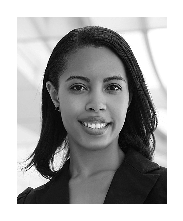
\includegraphics[width=1in,height=1.25in,clip,keepaspectratio]{a1.eps}}]{First A. Author} (M'76--SM'81--F'87) and all authors may include biographies. Biographies are often not included in conference-related papers. This author became a Member (M) of IEEE in 1976, a Senior Member (SM) in 1981, and a Fellow (F) in 1987. The first paragraph may contain a place and/or date of birth (list place, then date). Next, the author's educational background is listed. The degrees should be listed with type of degree in what field, which institution, city, state, and country, and year the degree was earned. The author's major field of study should be lower-cased. The second paragraph uses the pronoun of the person (he or she) and not the author's last name. It lists military and work experience, including summer and fellowship jobs. Job titles are capitalized. The current job must have a location; previous positions may be listed without one. Information concerning previous publications may be included. Try not to list more than three books or published articles. The format for listing publishers of a book within the biography is: title of book (publisher name, year) similar to a reference. Current and previous research interests end the paragraph. The third paragraph begins with the author's title and last name (e.g., Dr.\ Smith, Prof.\ Jones, Mr.\ Kajor, Ms.\ Hunter). List any memberships in professional societies other than the IEEE. Finally, list any awards and work for IEEE committees and publications. If a photograph is provided, it should be of good quality, and professional-looking. Following are two examples of an author's biography.
%\end{IEEEbiography}

%\begin{IEEEbiography}[{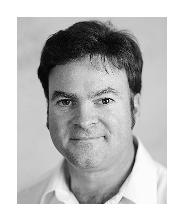
\includegraphics[width=1in,height=1.25in,clip,keepaspectratio]{a2.eps}}]{Second B. Author} was born in Greenwich Village, New York, NY, USA in 1977. He received the B.S. and M.S. degrees in aerospace engineering from the University of Virginia, Charlottesville, in 2001. Since 2009, he has been an Assistant Professor with the Mechanical Engineering Department, Texas A{\&}M University, College Station. He is the author of more than 150 articles. His research interests include high-pressure and high-density nonthermal plasma discharge processes and applications, plasma propulsion, and innovation plasma applications. Dr. Author was a recipient of the International Association of Geomagnetism and Aeronomy Young Scientist Award for Excellence in 2008, and the IEEE Electromagnetic  Compatibility Society Best Symposium Paper Award in 2011. 
%\end{IEEEbiography}

%\begin{IEEEbiography}[{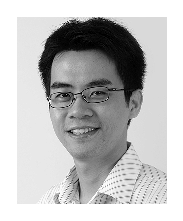
\includegraphics[width=1in,height=1.25in,clip,keepaspectratio]{a3.eps}}]{Third C. Author, Jr.} (M'87) received the B.S. degree in mechanical engineering from National Chung Cheng University, Chiayi, Taiwan, in 2004 and the M.S. degree in mechanical engineering from National Tsing Hua University, Hsinchu, Taiwan, in 2006. He is currently pursuing the Ph.D. degree in mechanical engineering at Texas A{\&}M University, College Station, TX, USA. From 2008 to 2009, he was a Research Assistant with the Institute of Physics, Academia Sinica, Tapei, Taiwan. His research interest includes the development of surface processing and biological/medical treatment techniques using nonthermal atmospheric pressure plasmas. Mr. Author's awards and honors include the Frew Fellowship (Australian Academy of Science), the I. I. Rabi Prize (APS), the European Frequency and Time Forum Award, the Carl Zeiss Research Award, the William F. Meggers Award and the Adolph Lomb Medal (OSA).
%\end{IEEEbiography}

\EOD

\end{document}
